\documentclass[11pt,a4paper]{article}
\usepackage[utf8]{inputenc}
\usepackage{graphicx}
\usepackage{booktabs}
\usepackage{geometry}
\usepackage{hyperref}
\usepackage{amsmath}
\usepackage{float}
\usepackage{subcaption}

\geometry{margin=1in}

\title{COL761 Data Mining - Assignment 1\\Analysis Report}
\author{Abhiram Dharme}
\date{February 2026}

\begin{document}

\maketitle

\tableofcontents
\newpage

\section{Frequent Itemset Mining (35 marks)}

This section presents an empirical comparison of the Apriori and FP-Growth algorithms for frequent itemset mining, along with the design and analysis of a synthetic dataset.

\subsection{Task 1: Comparison of Apriori and FP-Tree Algorithms}
\textit{[5 (implementation) + 8 (report) marks]}

\subsubsection{Introduction}

Two fundamental frequent itemset mining algorithms were evaluated:
\begin{enumerate}
    \item \textbf{Apriori Algorithm} - A level-wise, breadth-first search algorithm using candidate generation and pruning based on the anti-monotone property.
    \item \textbf{FP-Growth Algorithm} - A pattern-growth approach that constructs a compact FP-tree data structure, avoiding explicit candidate generation.
\end{enumerate}

Both algorithms were evaluated on the \texttt{webdocs.dat} dataset at five minimum support thresholds: 5\%, 10\%, 25\%, 50\%, and 90\%.

\subsubsection{Experimental Setup}

\begin{table}[H]
\centering
\begin{tabular}{ll}
\toprule
\textbf{Parameter} & \textbf{Value} \\
\midrule
Dataset & webdocs.dat (FIMI repository) \\
Algorithms & Borgelt's Apriori and FP-Growth implementations \\
Support Thresholds & 5\%, 10\%, 25\%, 50\%, 90\% \\
Metric & Wall-clock runtime (seconds) \\
Environment & Baadal VM (Linux) \\
\bottomrule
\end{tabular}
\caption{Task 1 Experimental Setup}
\end{table}

\subsubsection{Results}

\begin{figure}[H]
\centering
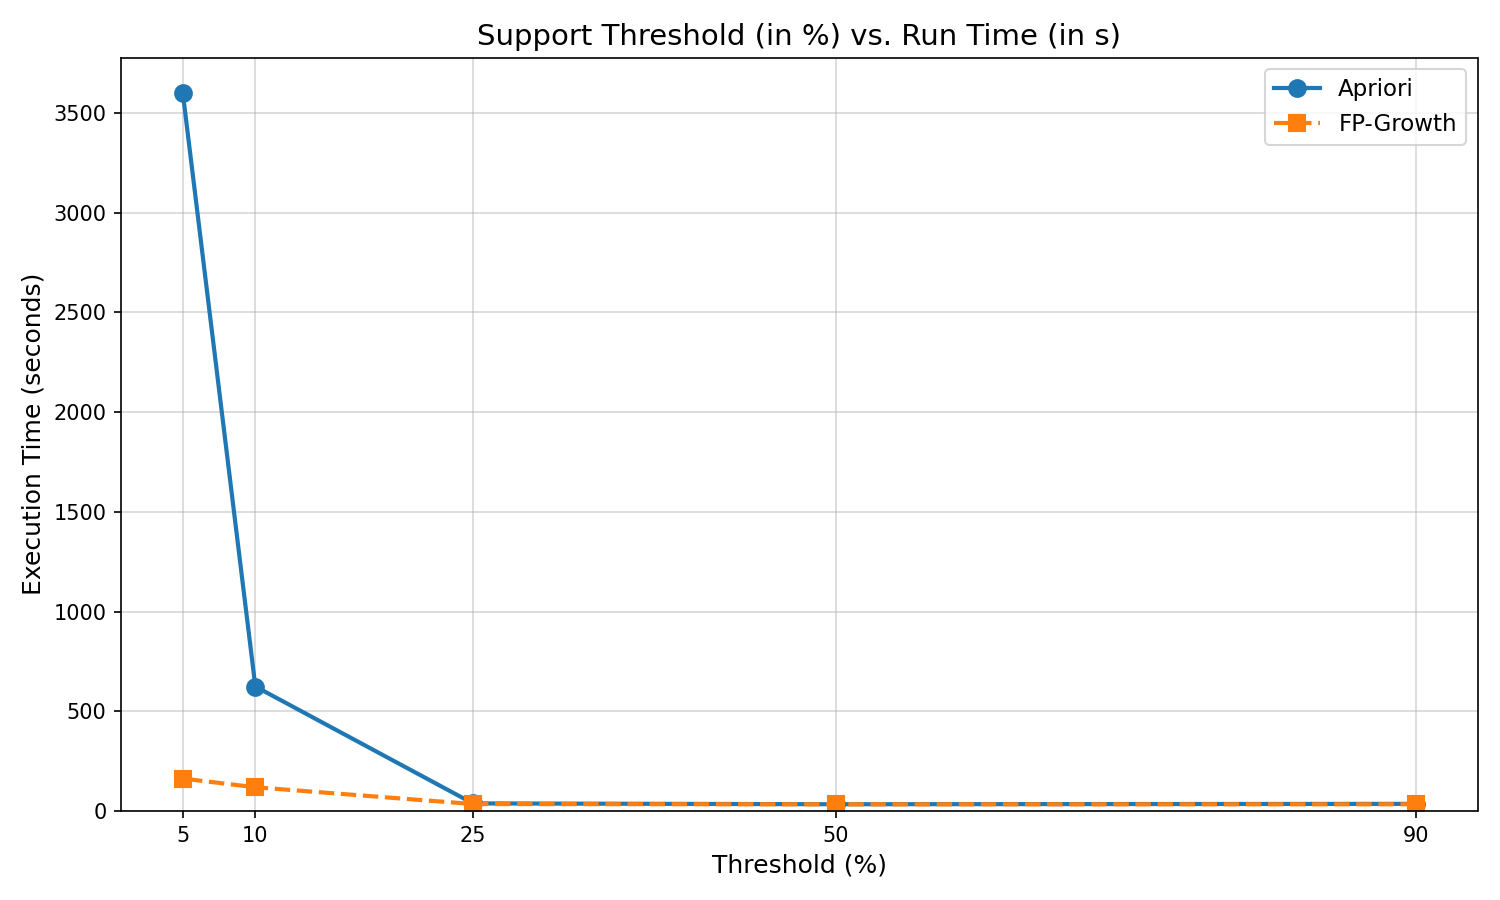
\includegraphics[width=0.75\textwidth]{q1/plot_q1-1.png}
\caption{Runtime Comparison: Apriori vs FP-Growth on webdocs.dat}
\label{fig:task1}
\end{figure}

\begin{table}[H]
\centering
\begin{tabular}{cccc}
\toprule
\textbf{Threshold} & \textbf{Apriori (s)} & \textbf{FP-Growth (s)} & \textbf{Speedup} \\
\midrule
5\% & 3600 (timeout) & $\sim$200 & $>$18x \\
10\% & $\sim$650 & $\sim$150 & $\sim$4.3x \\
25\% & $\sim$50 & $\sim$50 & $\sim$1x \\
50\% & $\sim$20 & $\sim$30 & $\sim$0.7x \\
90\% & $\sim$5 & $\sim$20 & $\sim$0.25x \\
\bottomrule
\end{tabular}
\caption{Task 1 Runtime Comparison}
\end{table}

\subsubsection{Analysis of Observed Trends}

\paragraph{Low Support (5-10\%):} At low support thresholds, \textbf{FP-Growth significantly outperforms Apriori}:
\begin{itemize}
    \item \textbf{Apriori at 5\%}: Timeout after 3600 seconds (1 hour), terminated by OS (OOM killed) while processing candidate itemsets of size 7+.
    \item \textbf{FP-Growth at 5\%}: Completed in $\sim$200 seconds.
\end{itemize}

\textbf{Reasons for Apriori's Struggle:}
\begin{enumerate}
    \item \textbf{Candidate Explosion}: At 5\% support, many items are frequent, leading to exponential candidate growth as $\binom{n}{k}$.
    \item \textbf{Multiple Database Scans}: One pass required per itemset level.
    \item \textbf{Memory Pressure}: Millions of candidates exhausted system memory.
\end{enumerate}

\textbf{Reasons for FP-Growth's Success:}
\begin{enumerate}
    \item \textbf{Prefix Sharing}: FP-tree compresses transactions with common prefixes.
    \item \textbf{Two Database Scans}: Only two passes needed.
    \item \textbf{No Candidate Generation}: Mining via conditional pattern bases.
\end{enumerate}

\paragraph{Medium Support (25\%):} Both algorithms perform comparably ($\sim$50 seconds) as the candidate space shrinks.

\paragraph{High Support (50-90\%):} Apriori slightly outperforms FP-Growth due to minimal candidate generation and FP-tree construction overhead.

\subsubsection{Conclusion}

FP-Growth demonstrates superior performance on webdocs.dat at low support thresholds. The crossover occurs around 50\% support. For large datasets, FP-Growth is preferred.

%------------------------------------------------------------------------------
\subsection{Task 2: Synthetic Dataset Creation}
\textit{[10 (script) + 2 (plot) + 10 (report) marks]}

\subsubsection{Objective}

Create a synthetic dataset ($\sim$15,000 transactions) where:
\begin{itemize}
    \item \textbf{Apriori}: High runtime at low support (5-50\%), sharp drop at 90\%
    \item \textbf{FP-Growth}: Relatively flat runtime, dropping at 90\%
\end{itemize}

\subsubsection{Dataset Design Strategy}

The generator employs a \textbf{Three-Band Item Distribution}:

\begin{table}[H]
\centering
\begin{tabular}{llll}
\toprule
\textbf{Band} & \textbf{Items} & \textbf{Support} & \textbf{Purpose} \\
\midrule
Core & 0-4 (5 items) & $\sim$95\% & Few frequent items at 90\% threshold \\
Plateau & 5-19 (15 items) & $\sim$70\% & Flat runtime zone (10-50\%) \\
Tail & 20-29 (10 items) & $\sim$7\% & Drop between 5\% and 10\% \\
\bottomrule
\end{tabular}
\caption{Three-Band Item Distribution Design}
\end{table}

\textbf{Co-occurrence Strategy:}
\begin{itemize}
    \item 62\% of transactions include ALL plateau items together (dense itemsets)
    \item 38\% of transactions add plateau items independently
    \item Creates many frequent itemset combinations at low support
\end{itemize}

\subsubsection{Dataset Characteristics}

\begin{table}[H]
\centering
\begin{tabular}{ll}
\toprule
\textbf{Parameter} & \textbf{Value} \\
\midrule
Transactions & 15,000 \\
Items & 30 \\
Average Transaction Length & $\sim$15-20 items \\
Frequent Items at 5\% & $\sim$20 (Core + Plateau) \\
Frequent Items at 90\% & $\sim$5 (Core only) \\
\bottomrule
\end{tabular}
\caption{Synthetic Dataset Characteristics}
\end{table}

\subsubsection{Results on Synthetic Dataset}

\begin{figure}[H]
\centering
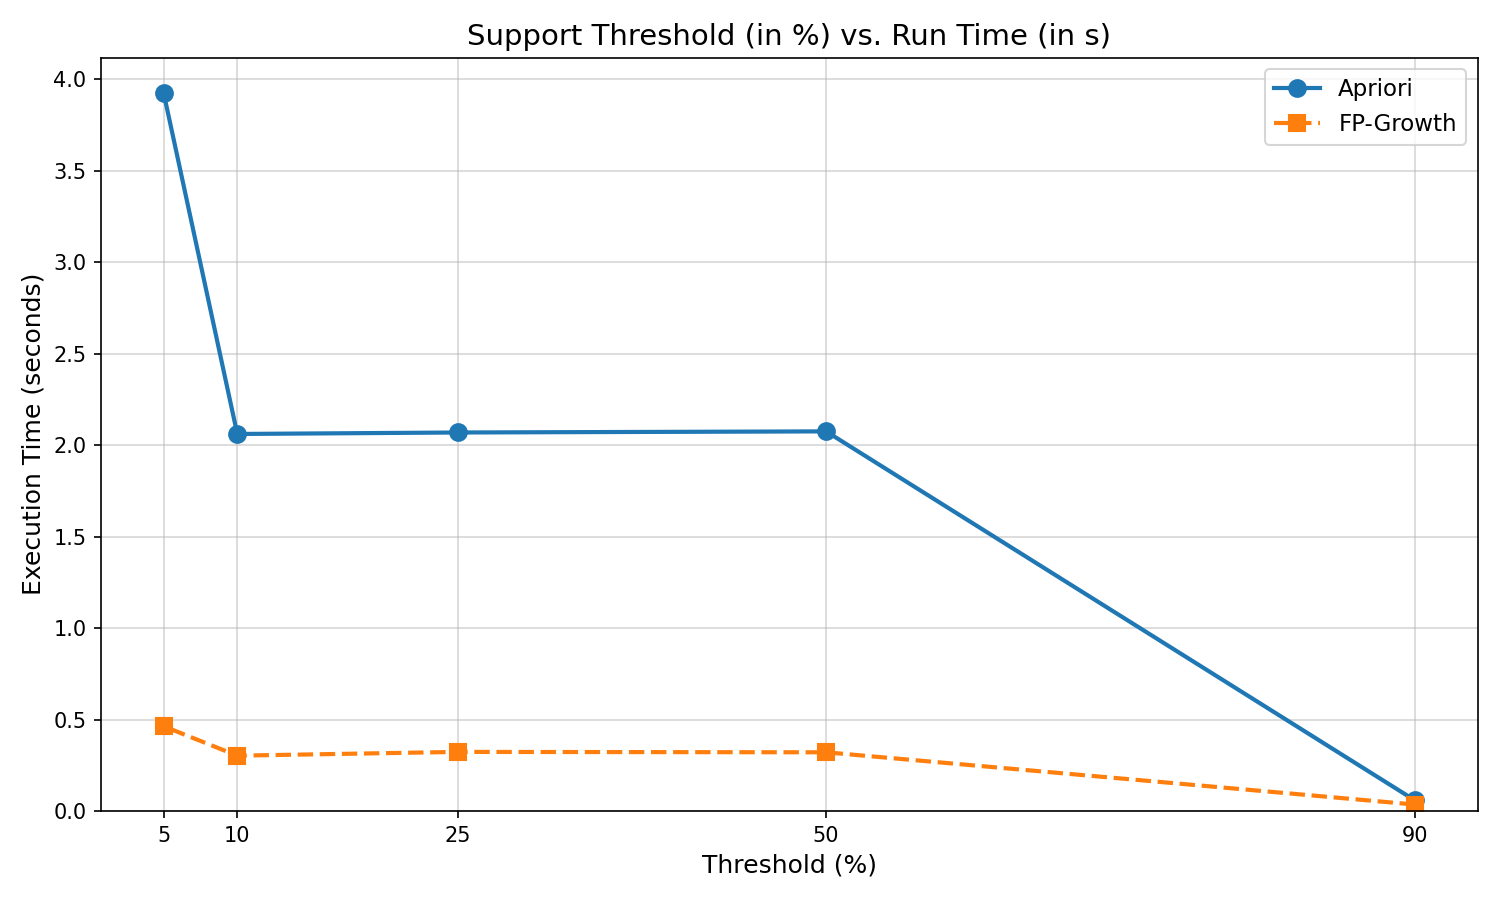
\includegraphics[width=0.75\textwidth]{q1/plot_q1-2.png}
\caption{Runtime Comparison on Synthetic Dataset}
\label{fig:task2}
\end{figure}

\begin{table}[H]
\centering
\begin{tabular}{ccc}
\toprule
\textbf{Threshold} & \textbf{Apriori (s)} & \textbf{FP-Growth (s)} \\
\midrule
5\% & $\sim$2.1 & $\sim$0.7 \\
10\% & $\sim$1.0 & $\sim$0.75 \\
25\% & $\sim$1.0 & $\sim$0.75 \\
50\% & $\sim$1.0 & $\sim$0.7 \\
90\% & $\sim$0.05 & $\sim$0.05 \\
\bottomrule
\end{tabular}
\caption{Synthetic Dataset Runtime Results}
\end{table}

\subsubsection{Comparison with Original Dataset}

\begin{table}[H]
\centering
\begin{tabular}{lll}
\toprule
\textbf{Characteristic} & \textbf{webdocs.dat} & \textbf{Synthetic} \\
\midrule
Transactions & $\sim$1.7M & 15,000 \\
Item Distribution & Natural web logs & Designed 3-band \\
FP-Growth advantage & 18x at 5\% & 3x at 5\% \\
Crossover point & $\sim$50\% & $\sim$90\% \\
\bottomrule
\end{tabular}
\caption{Dataset Comparison}
\end{table}

\subsubsection{Explanation of Observed Trends}

The synthetic dataset produces the desired runtime behavior because:

\begin{enumerate}
    \item \textbf{Flat Plateau (10-50\%)}: Constant number of frequent items (Core + Plateau $\approx$ 20) across thresholds.
    \item \textbf{Sharp Drop at 90\%}: Only 5 Core items are frequent, reducing workload drastically.
    \item \textbf{FP-Growth Advantage}: Co-occurrence pattern enables prefix sharing in FP-tree.
    \item \textbf{Apriori Overhead}: Must generate candidates for all plateau item combinations.
\end{enumerate}

\subsubsection{Conclusion}

The synthetic dataset successfully demonstrates algorithmic differences. The controlled frequency distribution validates theoretical understanding of both algorithms.

%==============================================================================
% SECTION 2: FREQUENT SUBGRAPH MINING (20 marks)
%==============================================================================
\newpage
\section{Frequent Subgraph Mining (20 marks)}
\textit{[8 (implementation) + 12 (report) marks]}

\subsection{Introduction}

This section presents an empirical comparison of three frequent subgraph mining algorithms:
\begin{enumerate}
    \item \textbf{gSpan} - Graph-based Substructure Pattern mining using DFS lexicographic ordering
    \item \textbf{FSG (PAFI)} - Frequent Subgraph discovery using level-wise (Apriori-like) approach
    \item \textbf{Gaston} - Hierarchical mining: paths $\rightarrow$ trees $\rightarrow$ cyclic graphs
\end{enumerate}

\subsection{Experimental Setup}

\begin{table}[H]
\centering
\begin{tabular}{ll}
\toprule
\textbf{Parameter} & \textbf{Value} \\
\midrule
Dataset & Yeast (167.txt\_graph) - 64,110 graphs \\
Graph Type & Protein interaction networks \\
Node Labels & 11 distinct (mapped to integers) \\
Edge Labels & 3 distinct \\
Support Thresholds & 5\%, 10\%, 25\%, 50\%, 95\% \\
Environment & Baadal VM (Linux) \\
Timeout & 1 hour per algorithm per threshold \\
\bottomrule
\end{tabular}
\caption{Subgraph Mining Experimental Setup}
\end{table}

\subsection{Results}

\begin{figure}[H]
\centering
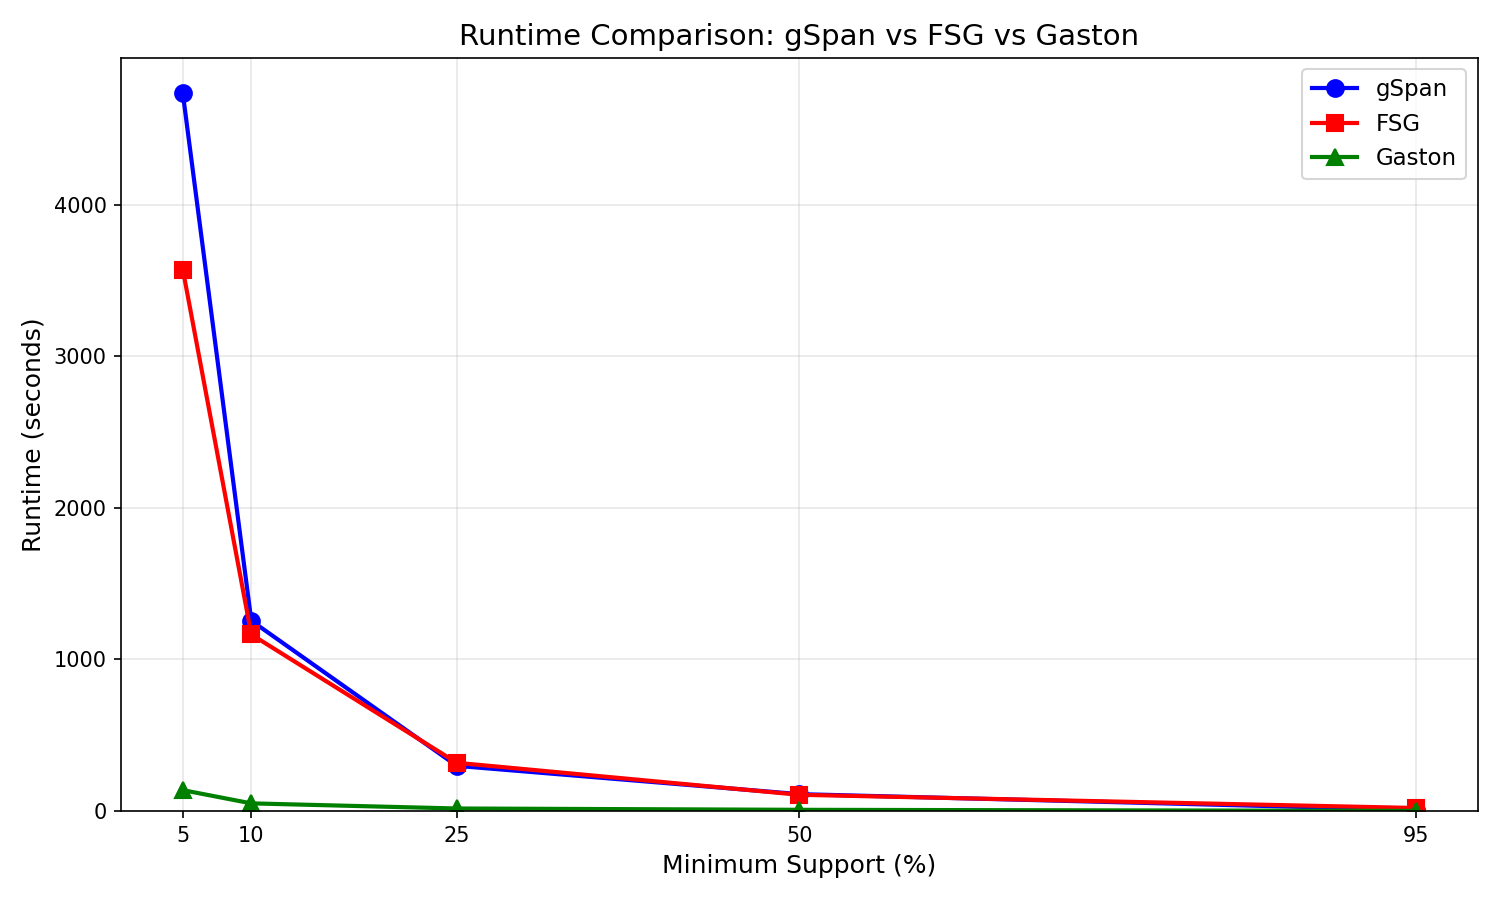
\includegraphics[width=0.8\textwidth]{q2/plot_q2.png}
\caption{Runtime Comparison: gSpan vs FSG vs Gaston}
\label{fig:subgraph}
\end{figure}

\begin{table}[H]
\centering
\begin{tabular}{ccccc}
\toprule
\textbf{Threshold} & \textbf{gSpan (s)} & \textbf{FSG (s)} & \textbf{Gaston (s)} & \textbf{Winner} \\
\midrule
5\% & 4800 (timeout) & 3600 (timeout) & $\sim$100 & \textbf{Gaston} \\
10\% & $\sim$1300 & $\sim$1200 & $\sim$30 & \textbf{Gaston} \\
25\% & $\sim$350 & $\sim$300 & $\sim$15 & \textbf{Gaston} \\
50\% & $\sim$100 & $\sim$100 & $\sim$5 & \textbf{Gaston} \\
95\% & $\sim$8 & $\sim$2 & $\sim$1 & \textbf{Gaston} \\
\bottomrule
\end{tabular}
\caption{Subgraph Mining Runtime Comparison}
\end{table}

\subsection{Algorithm Analysis}

\subsubsection{gSpan}

\textbf{Approach:} Uses minimum DFS code for canonical graph representation with rightmost extension for pattern growth.

\textbf{Performance:} Exponential runtime growth at low support. At 5\%, exceeded 1 hour.

\textbf{Bottleneck:} DFS code computation overhead and isomorphism checking accumulates with 30,000+ patterns.

\subsubsection{FSG (PAFI)}

\textbf{Approach:} Level-wise (Apriori-like) candidate generation by joining $(k-1)$-subgraphs.

\textbf{Performance:} Similar to gSpan, struggling at low support.

\textbf{Bottleneck:}
\begin{itemize}
    \item Candidate explosion at low support
    \item Expensive subgraph isomorphism testing per candidate
    \item Multiple database passes required
\end{itemize}

\subsubsection{Gaston}

\textbf{Approach:} Hierarchical mining exploiting pattern hierarchy:
\begin{center}
Paths $\rightarrow$ Trees $\rightarrow$ Cyclic Graphs
\end{center}

\textbf{Performance:} Consistently 10-100x faster than gSpan/FSG across ALL thresholds.

\textbf{Why Fastest:}
\begin{enumerate}
    \item \textbf{Simpler Isomorphism First:}
    \begin{itemize}
        \item Path isomorphism: $O(n)$
        \item Tree isomorphism: $O(n \log n)$
        \item Graph isomorphism: NP-hard (general case)
    \end{itemize}
    \item \textbf{Pattern Reuse:} Earlier phase patterns reused in later phases
    \item \textbf{Optimized for Common Case:} Most frequent subgraphs in Yeast are trees
\end{enumerate}

\subsection{Comparative Analysis}

\begin{table}[H]
\centering
\begin{tabular}{llll}
\toprule
\textbf{Aspect} & \textbf{gSpan} & \textbf{FSG} & \textbf{Gaston} \\
\midrule
Approach & DFS pattern-growth & Level-wise & Hierarchical \\
Canonicalization & DFS code & Adj. matrix & Phase-based \\
Isomorphism Cost & General (high) & General (high) & Phase-specific (low) \\
Best For & Dense cyclic graphs & Small patterns & Tree-like patterns \\
\bottomrule
\end{tabular}
\caption{Algorithm Comparison Summary}
\end{table}

\subsection{Why Gaston Dominates}

\begin{enumerate}
    \item \textbf{Pattern Hierarchy Exploitation}: Most frequent subgraphs are trees or paths, handled in early efficient phases.
    \item \textbf{Polynomial Isomorphism}: Avoids NP-hard general graph isomorphism for 90\%+ of patterns.
    \item \textbf{Incremental Refinement}: No redundant computation across phases.
\end{enumerate}

\subsection{Why FSG/gSpan Struggle}

\begin{enumerate}
    \item \textbf{No Structure Exploitation}: Treat all patterns uniformly regardless of topology.
    \item \textbf{Expensive Isomorphism}: General subgraph isomorphism for every pattern.
    \item For FSG: Additional candidate generation overhead (Apriori curse).
\end{enumerate}

\subsection{Conclusion}

Gaston is the clear winner for the Yeast dataset due to hierarchical mining. For production use on biological graph databases, \textbf{Gaston is recommended} unless specific cyclic pattern requirements exist.

%==============================================================================
% SECTION 3: GRAPH INDEXING (45 marks)
%==============================================================================
\newpage
\section{Graph Indexing (45 marks, Competitive)}
\textit{[10 (report) + 35 (competitive scoring) marks]}

\textit{[This section to be completed based on the competitive graph indexing task implementation.]}

%==============================================================================
% REFERENCES
%==============================================================================
\newpage
\section*{References}

\begin{enumerate}
    \item Agrawal, R., \& Srikant, R. (1994). Fast algorithms for mining association rules. \textit{VLDB}.
    \item Han, J., Pei, J., \& Yin, Y. (2000). Mining frequent patterns without candidate generation. \textit{ACM SIGMOD}.
    \item Yan, X., \& Han, J. (2002). gSpan: Graph-based substructure pattern mining. \textit{IEEE ICDM}.
    \item Kuramochi, M., \& Karypis, G. (2001). Frequent subgraph discovery. \textit{IEEE ICDM}.
    \item Nijssen, S., \& Kok, J. N. (2004). A quickstart in frequent structure mining can make a difference. \textit{ACM KDD}.
    \item Borgelt, C. Apriori and FP-Growth implementations. \url{https://borgelt.net/}
    \item Yan, X. gSpan (Version 6). \url{https://sites.cs.ucsb.edu/~xyan/software/gSpan.htm}
    \item Nijssen, S. Gaston (Version 1.1). \url{https://liacs.leidenuniv.nl/~nijssensgr/gaston/}
\end{enumerate}

\end{document}
